%%%%%%%%%%%%%%%%%%%%%%%%%%%%%%%%%%%%%%%%%%%%%%%%%%%%%%%%%%%%%%%%%%%%%%%%%%%%%%%%
%2345678901234567890123456789012345678901234567890123456789012345678901234567890
%        1         2         3         4         5         6         7         8

\documentclass[letterpaper, 10 pt, conference]{ieeeconf}  % Comment this line out if you need a4paper

%\documentclass[a4paper, 10pt, conference]{ieeeconf}      % Use this line for a4 paper

\IEEEoverridecommandlockouts                              % This command is only needed if 
                                                          % you want to use the \thanks command

\overrideIEEEmargins                                      % Needed to meet printer requirements.

% See the \addtolength command later in the file to balance the column lengths
% on the last page of the document

% The following packages can be found on http:\\www.ctan.org
%\usepackage{graphics} % for pdf, bitmapped graphics files
%\usepackage{epsfig} % for postscript graphics files
%\usepackage{mathptmx} % assumes new font selection scheme installed
%\usepackage{times} % assumes new font selection scheme installed
%\usepackage{amsmath} % assumes amsmath package installed
%\usepackage{amssymb}  % assumes amsmath package installed

\usepackage[pdftex]{graphicx}
\usepackage{caption}
\usepackage{subcaption}
%\graphicspath{}
%\usepackage[utf8]{inputenc}
\usepackage{slashbox}
\setlength{\belowcaptionskip}{-8pt}
\usepackage{tikz}
\usetikzlibrary{shapes.geometric, arrows}


\tikzstyle{io} =[text centered, draw=black]
\tikzstyle{process} = [text centered, text width=1cm, draw=black]
\tikzstyle{arrow} = [thick,->,>=stealth]
\tikzstyle{darrow} = [thick,<->,>=stealth] 
\tikzstyle{io2} =[ text centered, draw=black]
\tikzstyle{process2} = [text width=2cm, draw=black]


\usepackage{paralist}
\usepackage{amsfonts}
\usepackage{hyperref}

\usepackage{url}
\usepackage{booktabs}


\usepackage{tikz}
\usetikzlibrary{positioning, calc}
\usetikzlibrary{shapes.geometric, arrows}

\usepackage{color}
\definecolor{lightgray}{rgb}{0.95, 0.95, 0.95}
\definecolor{darkgray}{rgb}{0.4, 0.4, 0.4}
%\definecolor{purple}{rgb}{0.65, 0.12, 0.82}
\definecolor{editorGray}{rgb}{0.95, 0.95, 0.95}
\definecolor{editorOcher}{rgb}{1, 0.5, 0} % #FF7F00 -> rgb(239, 169, 0)
\definecolor{editorGreen}{rgb}{0, 0.5, 0} % #007C00 -> rgb(0, 124, 0)
\definecolor{orange}{rgb}{1,0.45,0.13}		
\definecolor{olive}{rgb}{0.17,0.59,0.20}
\definecolor{brown}{rgb}{0.69,0.31,0.31}
\definecolor{purple}{rgb}{0.38,0.18,0.81}
\definecolor{lightblue}{rgb}{0.1,0.57,0.7}
\definecolor{lightred}{rgb}{1,0.4,0.5}


\usepackage[draft,nomargin,footnote]{fixme}

\graphicspath{{figs/}}

%\usepackage{xspace}

\title{\LARGE \bf
Child-Robot Spatial Arrangement in a Learning by Teaching Activity}


\author{Wafa Johal$^{1}$$^{2}$, Alexis Jacq$^{1}$$^{3}$, Ana Paiva$^{3}$ and Pierre Dillenbourg$^{1}$  % <-this % stops a space
\thanks{}% <-this % stops a space
\thanks{$^{1}$ CHILI Lab,
	$^{2}$ LSRO Lab,
        \'{E}cole F\'{e}d\'{e}rale Polytechnique Lausanne, Switzerland
        {\tt\small firstname.lastname@epfl.ch}}%
\thanks{$^{3}$Instituto Superior T\'{e}cnico, University of Lisbon, Portugal
        {\tt\small firstname.lastname@inesc-id.pt}}%
}


\begin{document}



\maketitle


%%%%%%%%%%%%%%%%%%%%%%%%%%%%%%%%%%%%%%%%%%%%%%%%%%%%%%%%%%%%%%%%%%%%%%%%%%%%%%%%
\begin{abstract}
In this paper, we present an experiment in the context of a child-robot interaction where we study the influence of the child-robot spatial arrangement on the child's focus of attention and the perception of the robot's performance. In the ``Co-Writer learning by teaching'' activity, the child teaches a Nao robot how to handwrite.
Usually only face-to-face spatial arrangements are tested in educational child robot interactions, but we explored two spatial conditions from Kendon's F-formation, the side-by-side and the face-to-face formations in a within subject experiment.
We estimated the gaze behaviour of the child and their consistency in grading the robot with regard to the robot's progress in writing. 
Even-though the demonstrations provided by children were not different between the two conditions (i.e. the robot's learning didn't differ),  the results showed that in the side-by-side condition children tended to be more indulgent with the robot's mistakes and to give it better feedback.
These results highlight the influence of experimental choices in child-robot interaction.
%These results will allow us to take into account the variability of the judgement of the children relatively to the robot's performances.
\end{abstract}


%%%%%%%%%%%%%%%%%%%%%%%%%%%%%%%%%%%%%%%%%%%%%%%%%%%%%%%%%%%%%%%%%%%%%%%%%%%%%%%%
\section{INTRODUCTION}

Application of robots in learning tasks has been increasing and has shown very promising results these past ten years. 
\emph{R-learning}, in reference to e-learning, aims to design robots that would be helpful for learning.
%In our research context, we consider the problem of how robots could enhance the effectiveness of education.
The potential of robots for individual adaptation and their physical ability makes them fit well in the educational world.
%todo on voi si on enleve
We investigate how robots can bring added value for learning by designing and selecting relevant physical tas and setting up the appropriate interaction.
In that vein, the Co-Writer projects aims to help children with difficulties in handwriting \cite{hood2015when}.
It is based on the idea of ``learning by teaching''.
Under this paradigm, by teaching a robot (Nao from Aldebaran) how to write, children learn and improve their handwriting at the same time.
The activity also plays with the \emph{protégé effect}, which makes children more engaged in practising for the robot than for themselves.

Previous studies in the Co-Writer project helped to develop a system that generates handwriting for the robot based on demonstrations from the child\cite{hood2015when}.
Case studies presented in \cite{jacq2016building} showed that children were able to stay engaged in long term interactions with repeated sessions within the Co-Writer activity in real pedagogical/therapeutic contexts.
These works proved to have a positive effect on the extrinsic motivation of the children when practicing their handwriting, thanks to the protégé effect.

Authors in \cite{Matsuzoe2012} had a similar approach to learning by teaching with their Care Receiving Robot, who was being taken care of and taught by a child using physical interaction. 
In this study, authors chose to investigate handwriting (or drawing shapes) as well, but with a more physical based approach.
In their experimental setting, the child would teach handwriting to the robot by placing himself behind the robot and moving it's hand.
This study varied from other works in educational human-robot interaction in a way that the child was not only facing the robot but would act as a care-taker rather than a teacher.

As robots are entering our living space, they must adapt to our social norms.
These norms vary from politeness to unspoken social rules (as for instance, the personal space of a person).
In home environments, robots will be expected to perform their functions in a manner that is clearly understandable and predictable by the humans around.
This requires adaptive personalization of the robot to the individual needs of the humans, but also to the task being currently performed.
Some previous studies showed that the spatial setting with a robot was also a way to convey non-verbal messages and it serves to influence the relationship with the user\cite{Takayama2009,kristoffersson2013measuring}. 
Spatial arrangement is still a factor relatively unexplored in HRI and its influence on the interaction is still unclear. 

In this study, we explore the effect of spatial arrangement on the child-robot interaction within the Co-Writer activity.

\section{RELATED WORKS}
Spatial configuration is part of non-verbal cues of interpersonal stance.
Spatial arrangement is also a social signal that tells about the relationship between people.
Kendon \cite{Kendon2010} called the F-Formation a spatial-orientational system that aims to explain how people arrange themselves in a group interaction.
%According to Kendon, the way people arrangement themselves during an interaction reflects their engagement and involvement with the other persons. 
Kendon proposed three main F-formations : face-to-face (or vis-a-vis), L shape and side-by-side. These formations are illustrated by Figure \ref{fig:fformations}.
\begin{figure}[h!]
	\centering
	\begin{subfigure}{0.2\textwidth}
		\centering
		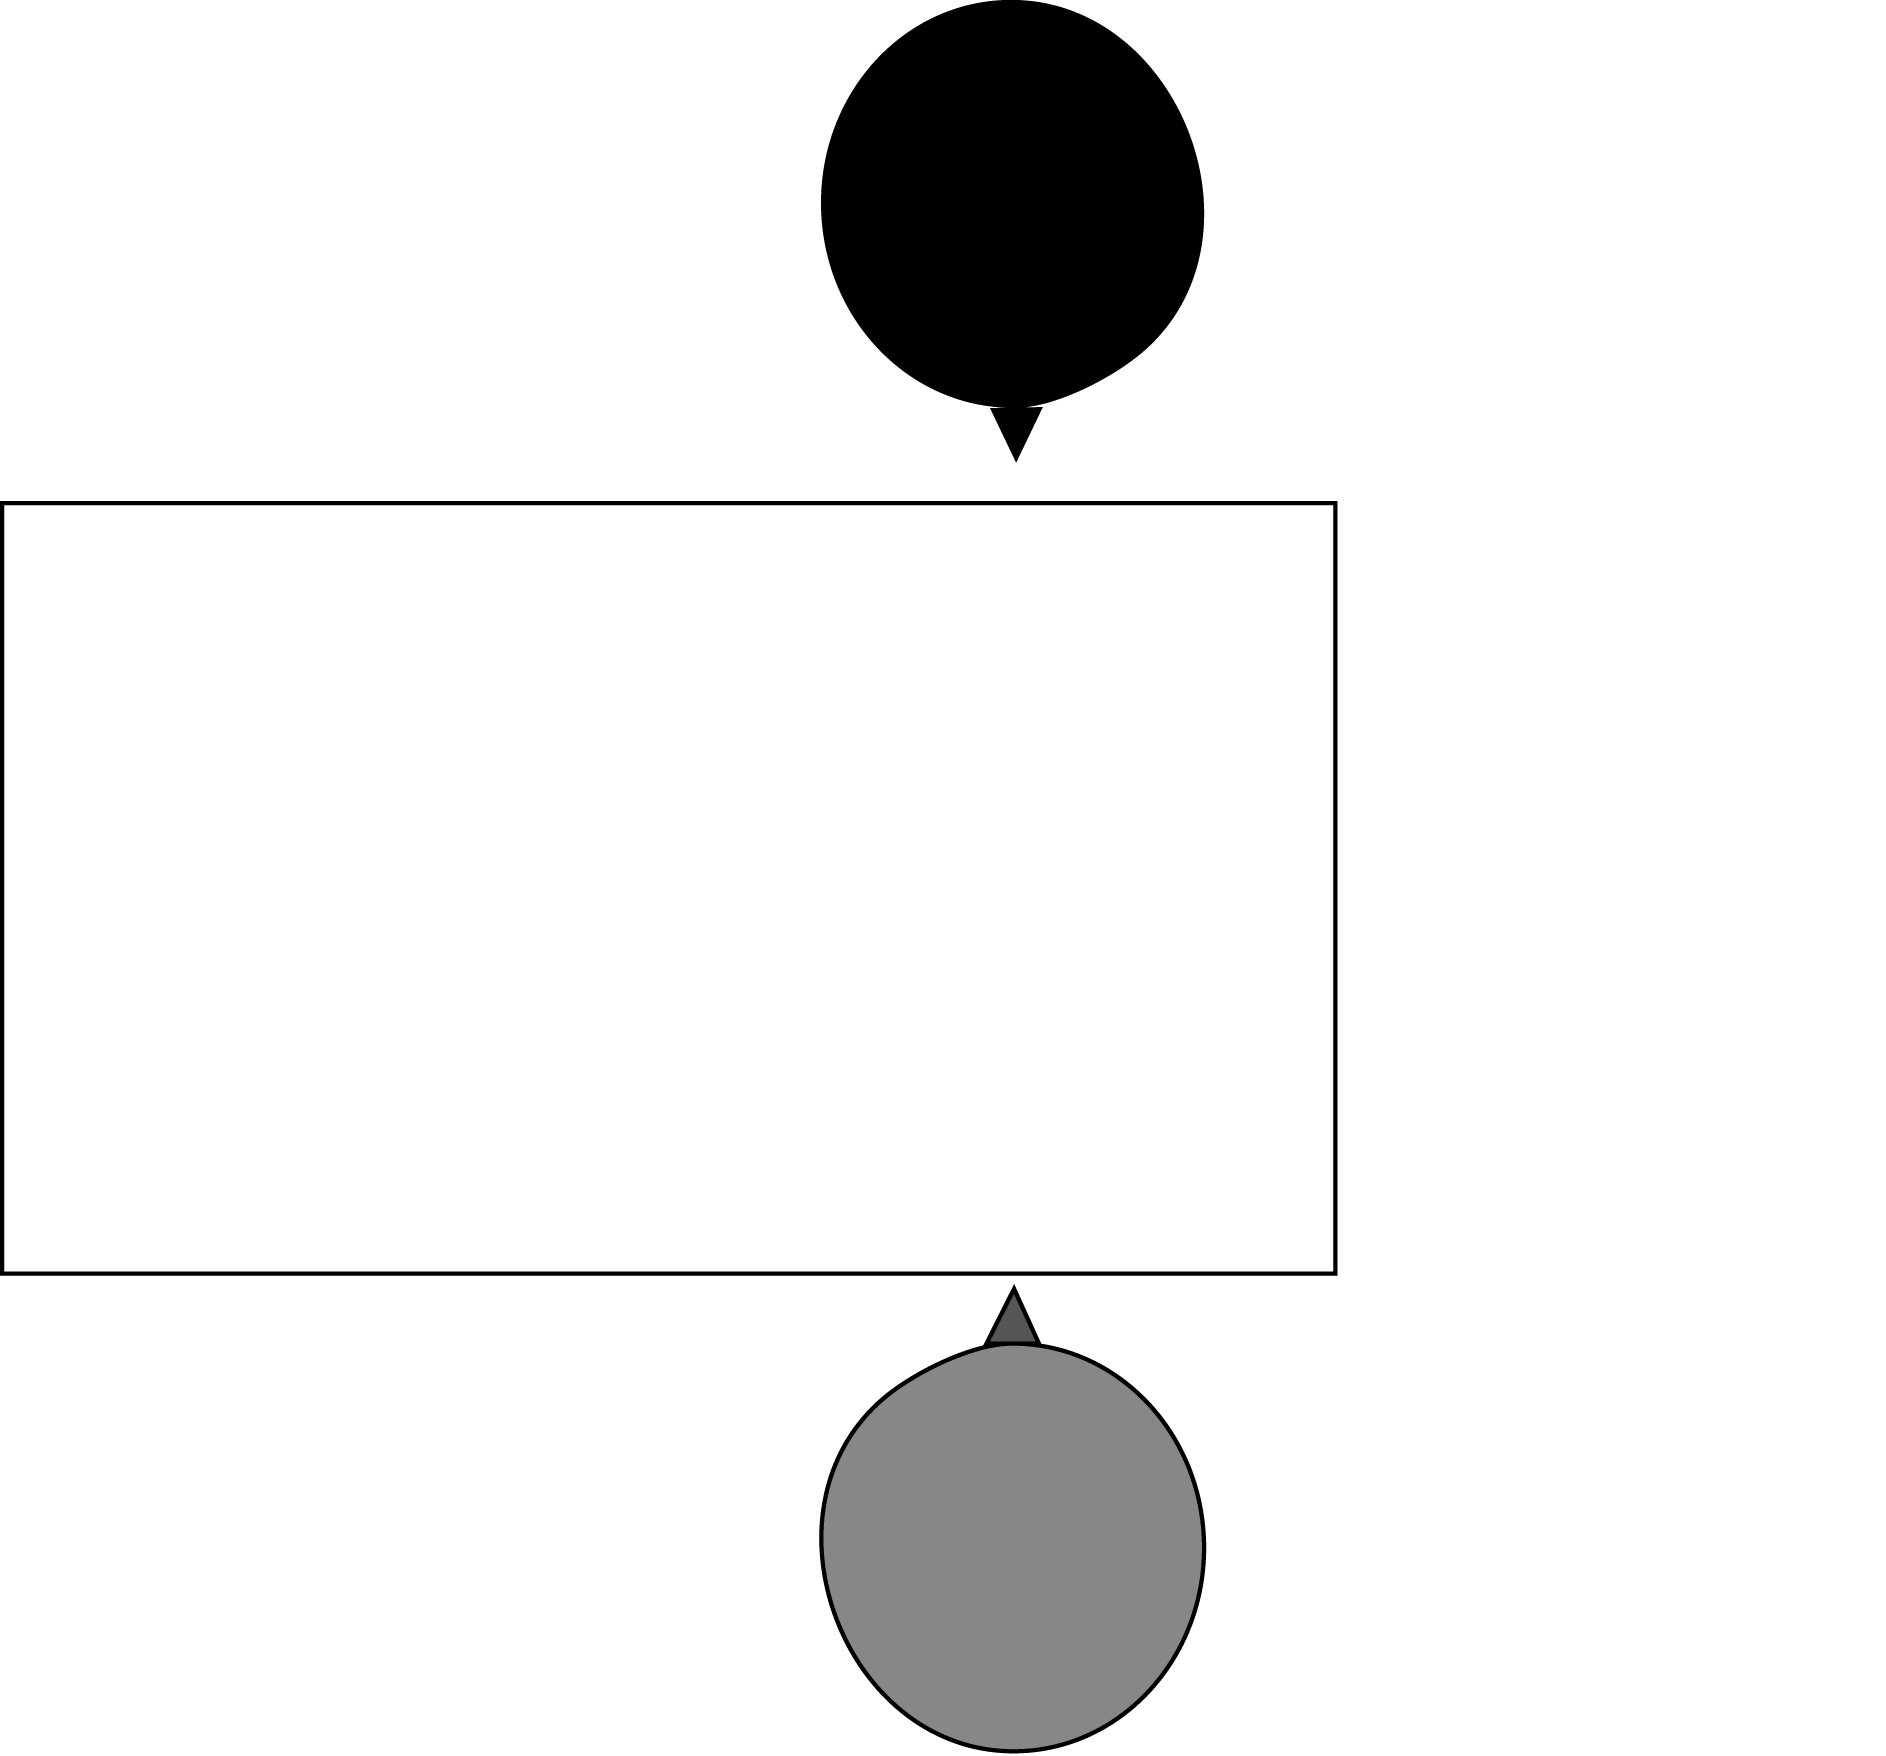
\includegraphics[width=0.75\linewidth]{./figures/fformationff.png}
		\caption{Face to face}
		\label{fig:ff}
	\end{subfigure}%
	\begin{subfigure}{0.2\textwidth}
		\centering
		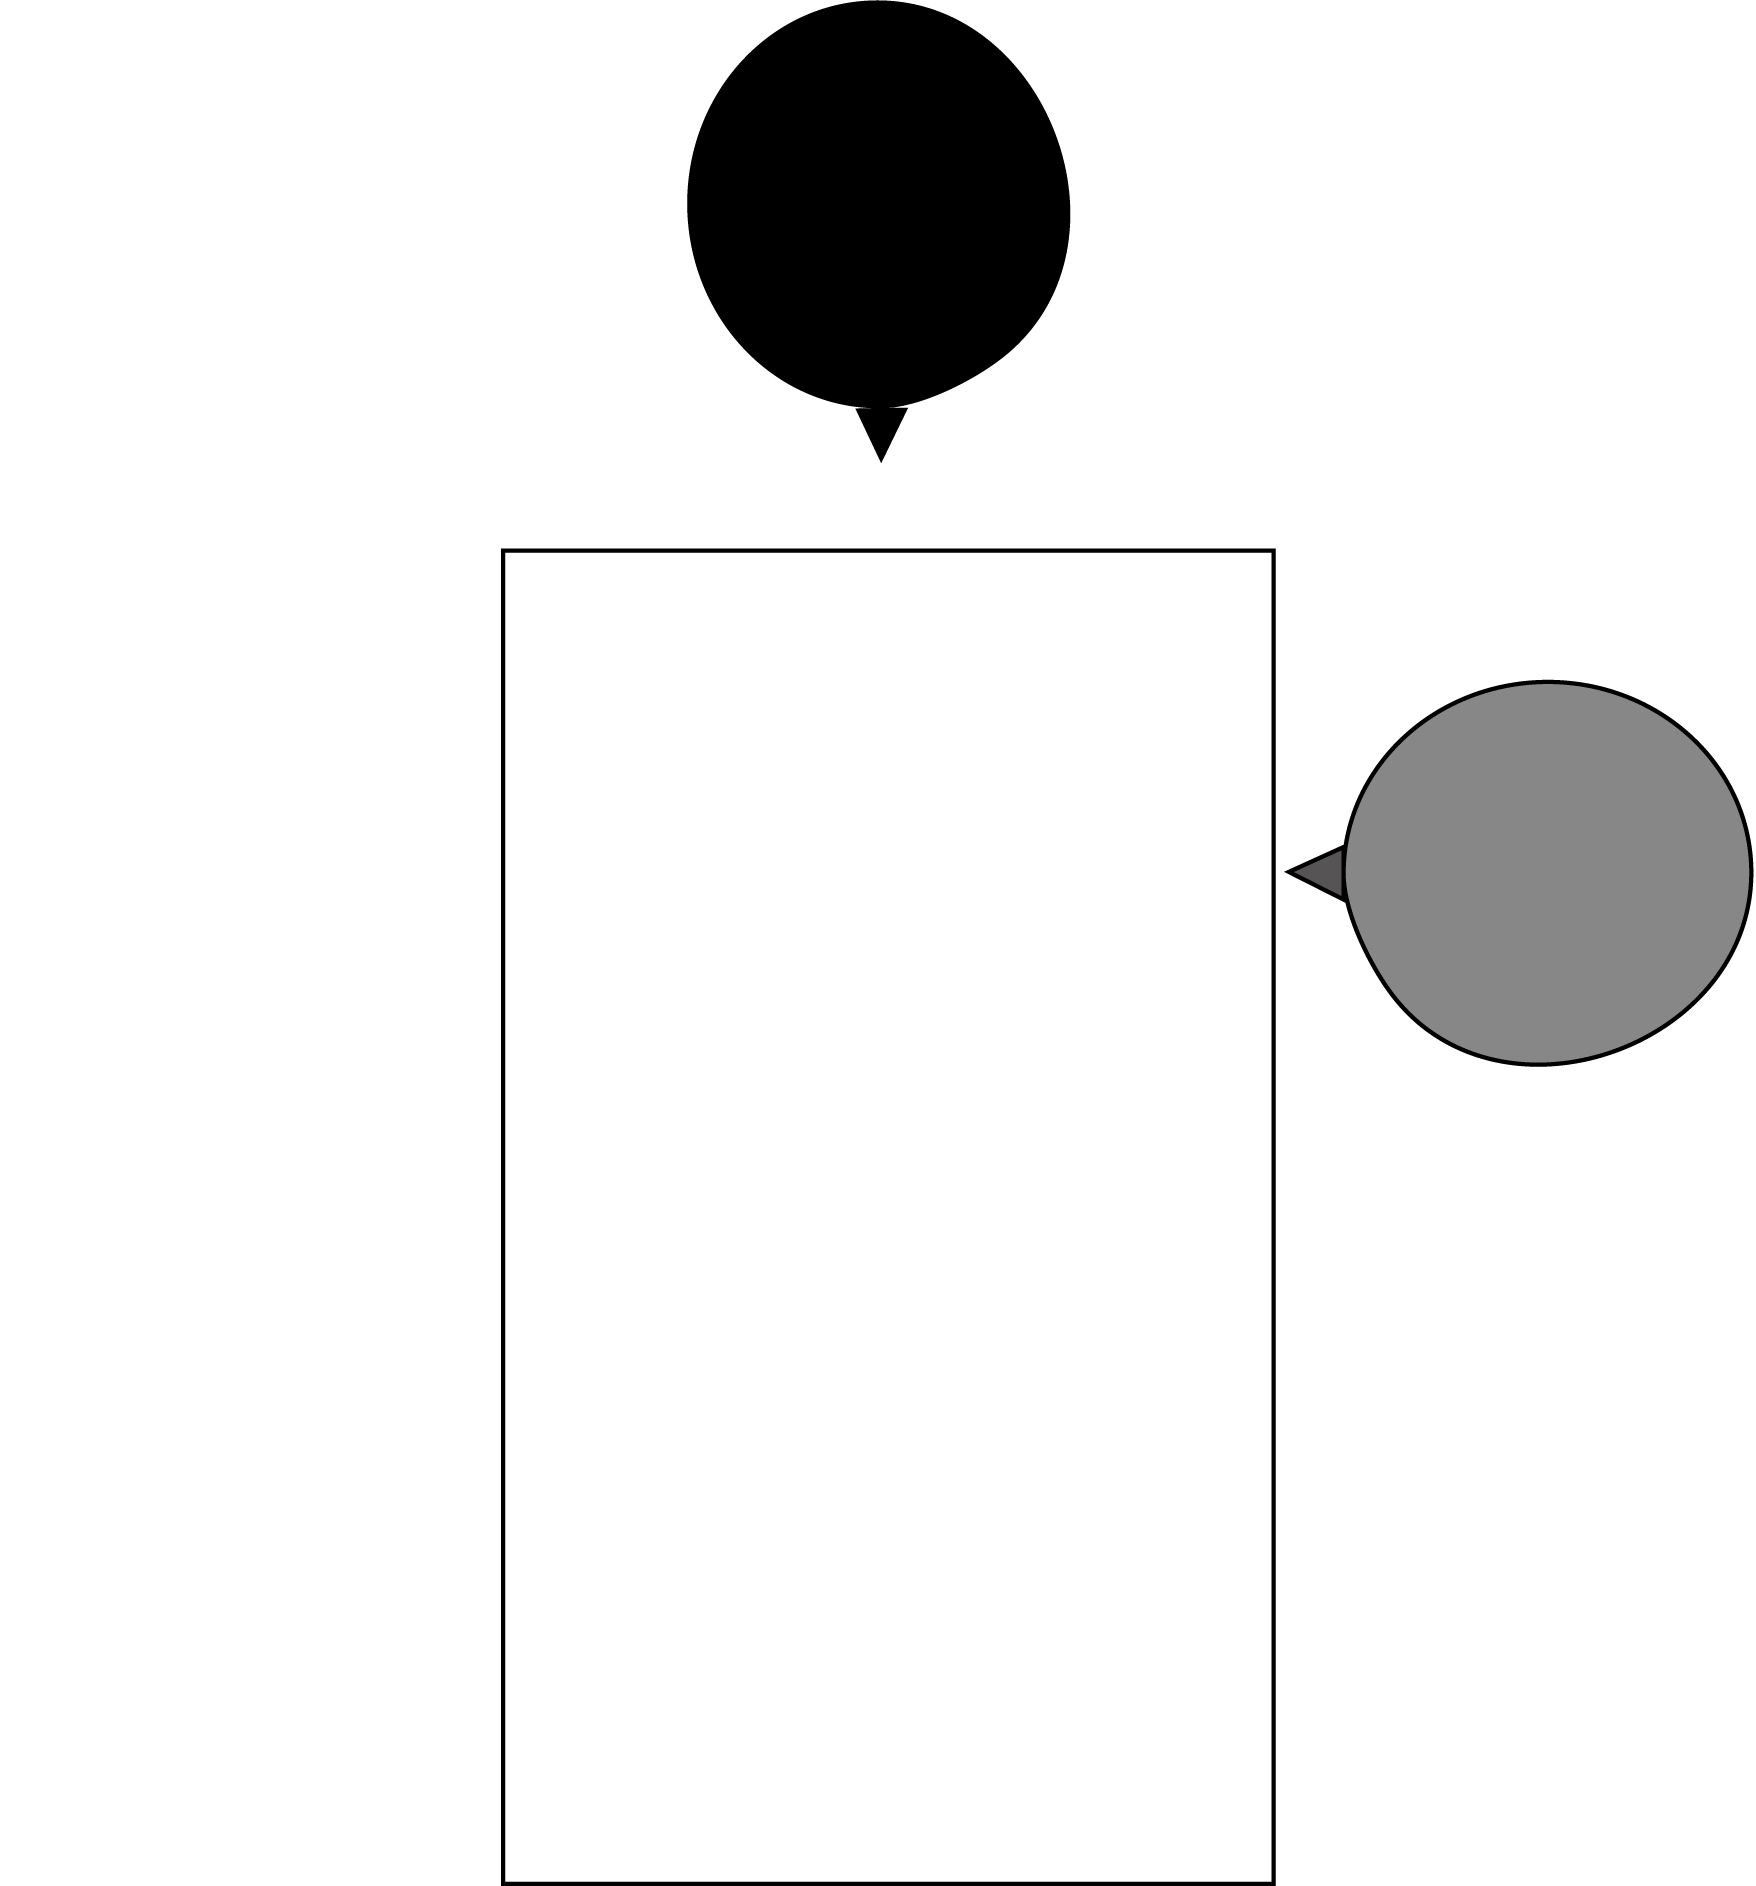
\includegraphics[width=0.75\linewidth]{./figures/fformationL.png}
		\caption{L-Shape}
		\label{fig:lshape}
	\end{subfigure}
	\begin{subfigure}{0.2\textwidth}
		\centering
		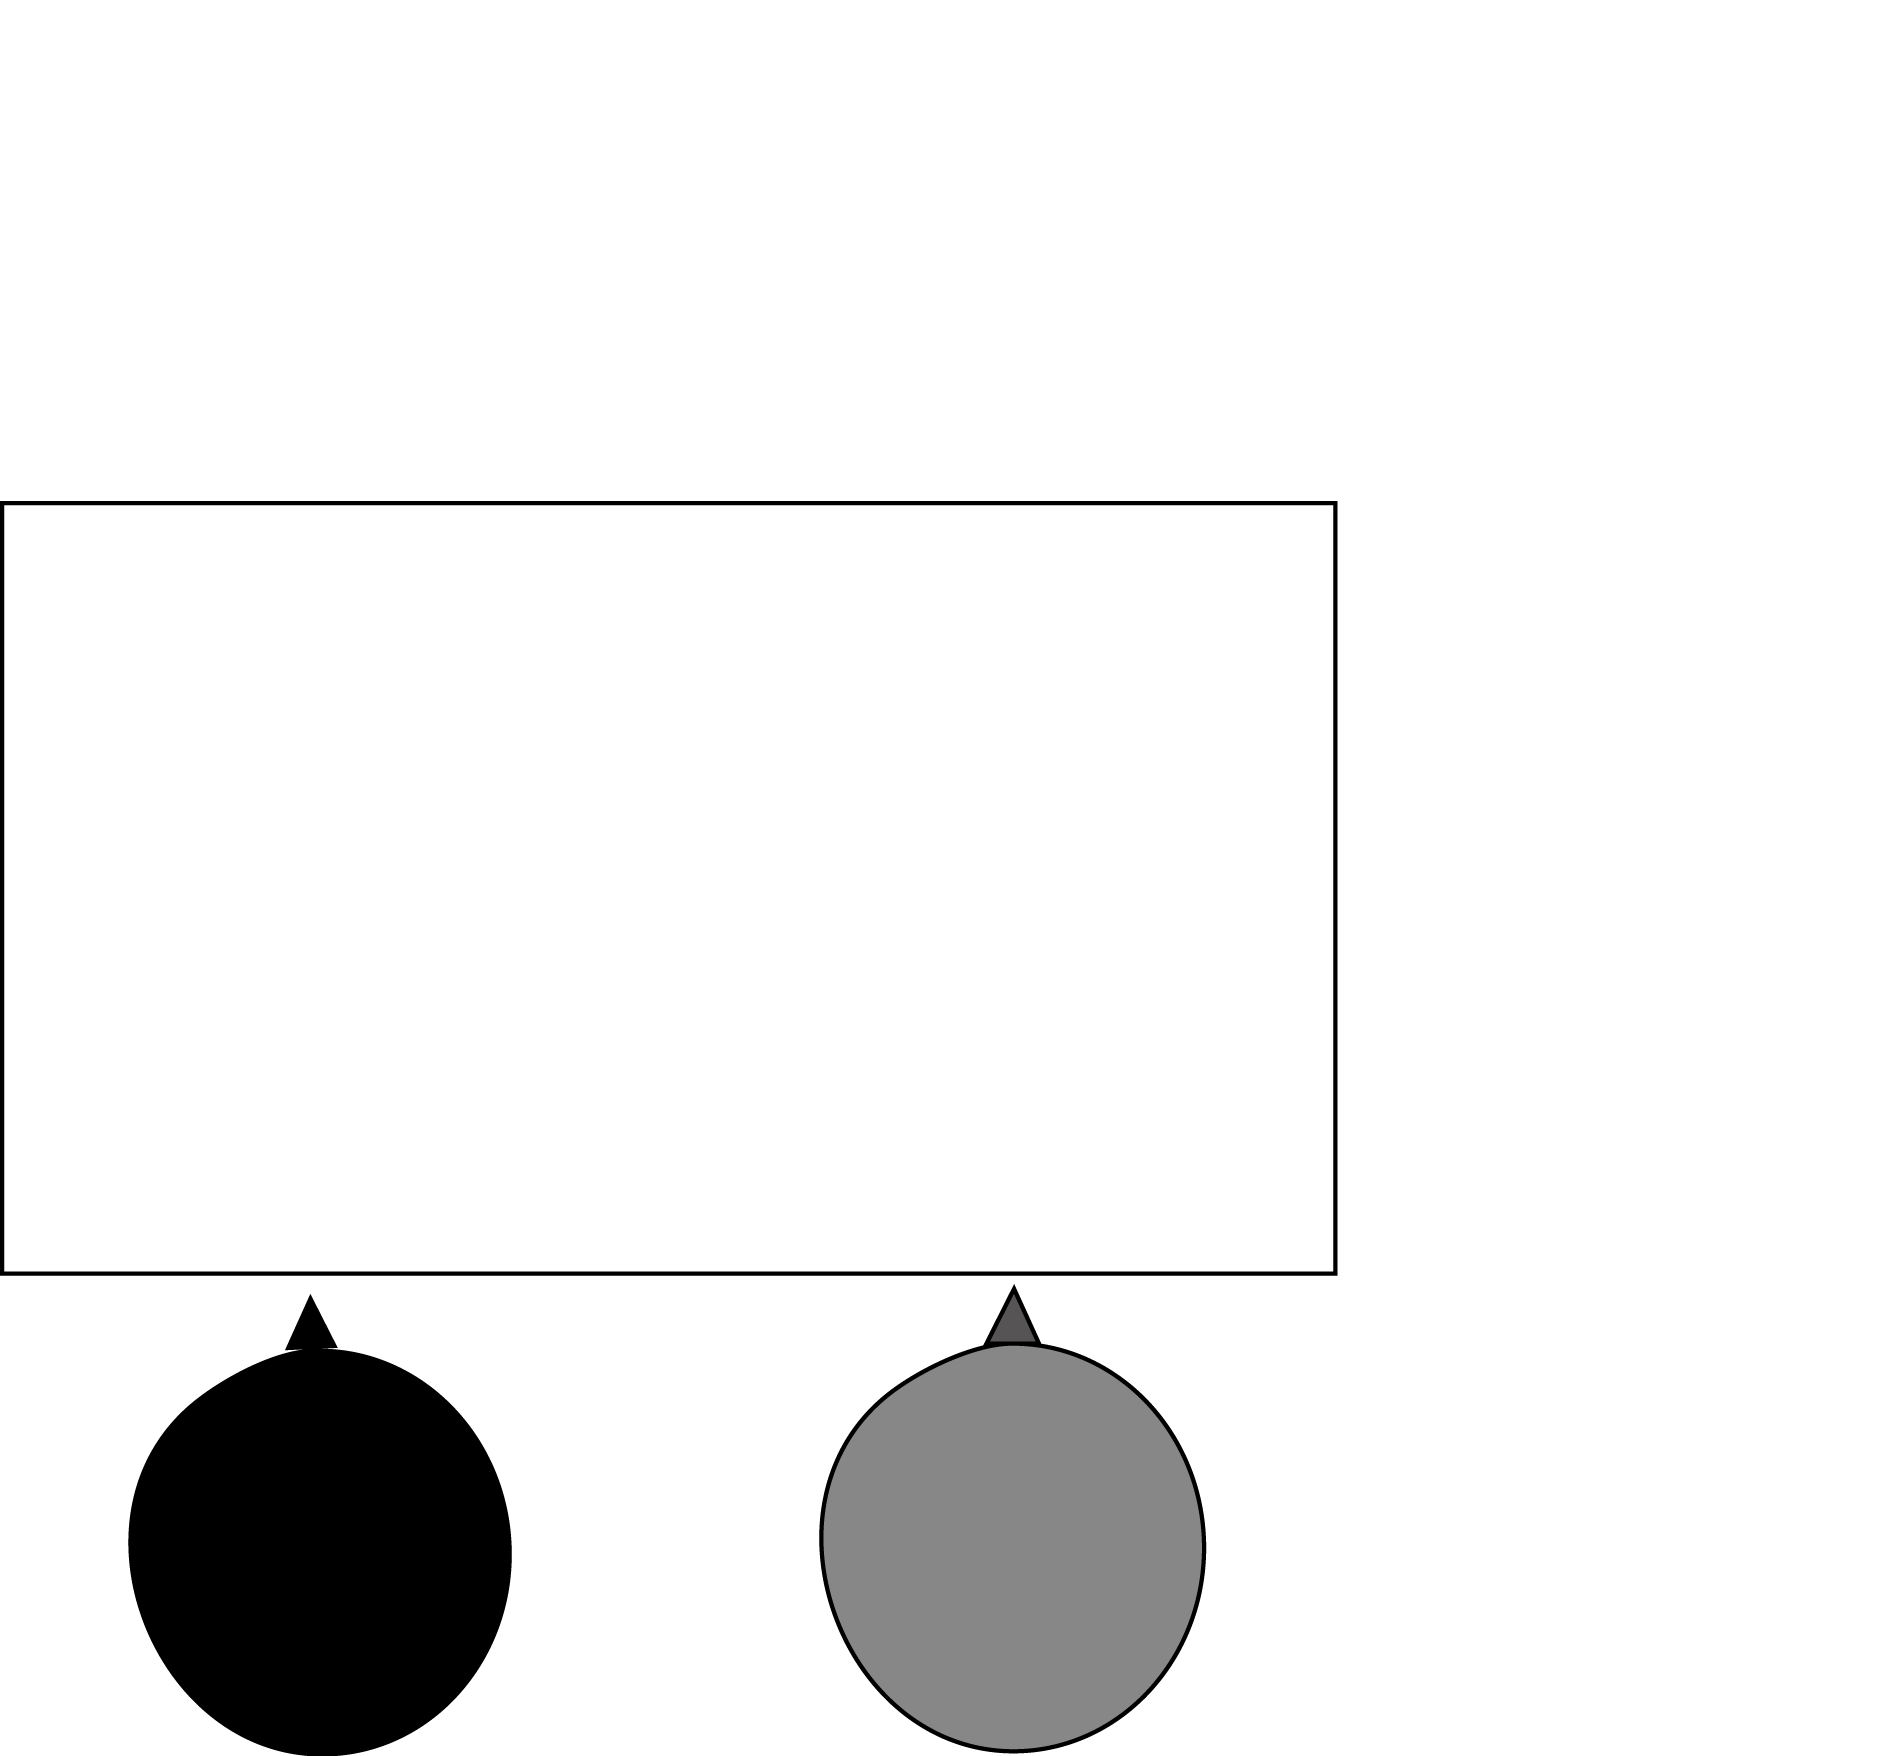
\includegraphics[width=0.75\linewidth]{./figures/fformationss.png}
		\caption{Side by Side }
		\label{fig:sidebside}
	\end{subfigure}
	\caption{Three possible Kendon's F-formations around a rectangular table}
	\label{fig:fformations}
\end{figure}

According to \cite{knapp2013nonverbal}, spatial arrangement and seating position can determine a person's role in a group.
It could also predispose the person to either competitive (face to face) or cooperative (side by side) mental setting in a shared task.



In educational child-robot interaction, quite often, the robot is placed in front of the learner playing the role of a tutor or a peer helping the child, and uses social capabilities to enhance the learning \cite{Saerbeck2010}.
Kanda \cite{Kanda2004} reported an experiment involving children that learns from a robot as they would from a peer.
In this other experiment,
\cite{Leyzberg2014} showed in a face-to-face setting that the physical presence of the robot produced measurable learning gains.
\cite{Kennedy2015} confirmed these results but recommended caution when applying social behaviors in a tutoring context. 
%explain why caution

Spatial arrangements have been studied in previous research\cite{Kuzuoka,huttenrauch2006investigating,vazquez2014spatial} in HRI, often as a challenge of path planning, or as a metric but less frequently as a non-verbal cue of communication in a learning task.

We propose to study the impact of spatial arrangement on the engagement of children in a handwriting task.
We performed a study in a school with 12 children performing the same teaching task under two conditions.
The child was either facing the robot (similar to other tutoring experiments) or was sitting next to the robot (as a peer teaching setup).


\section{METHOD}
The experiment took place in a primary school in Switzerland where children are taught in English.
In this experiment, we targeted children aged 5 y.o. who start handwriting, but do not typically master it yet.
The children interacted with the robot under two conditions of the F-Formation in a counterbalanced manner.

Our goal was to investigate the effect of spatial arrangement on the interaction.
We expected that children would give better feedback(see \ref{ss:feedback}) to the robot
when teaching it in a side-by-side configuration for several reasons.
The side-by-side arrangement corresponds to a cooperative arrangement which is close to a peer teaching setting, unlike the face-to-face teaching arrangement, which is more frequent seen in competitive or conversation tasks (closer to a teacher-student relationship).
Also, in the side-by-side formation, the robot and the child have the same visual perspective of the shared tablet on which they write.
Perspective sharing is an ability that facilitates mutual understanding \cite{berlin2006perspective}.
Hence by having the robot and the child side-by-side, higher mutual understanding would be expected.

\subsection{Participants and Apparatus}
12 subjects (six girls) from the same classroom (aged 5 to 6 y.o.) participated to the within subject study.
The two considered F-formations for this experiment are presented in the Figure~\ref{fig:test}: face-to-face~\ref{fig:sub1} and side-by-side~\ref{fig:sub2}.
Children were presented the two conditions sequentially with and interval of three days in a counterbalanced manner.

\begin{figure*}
\centering
\begin{subfigure}{0.5\textwidth}
  \centering
  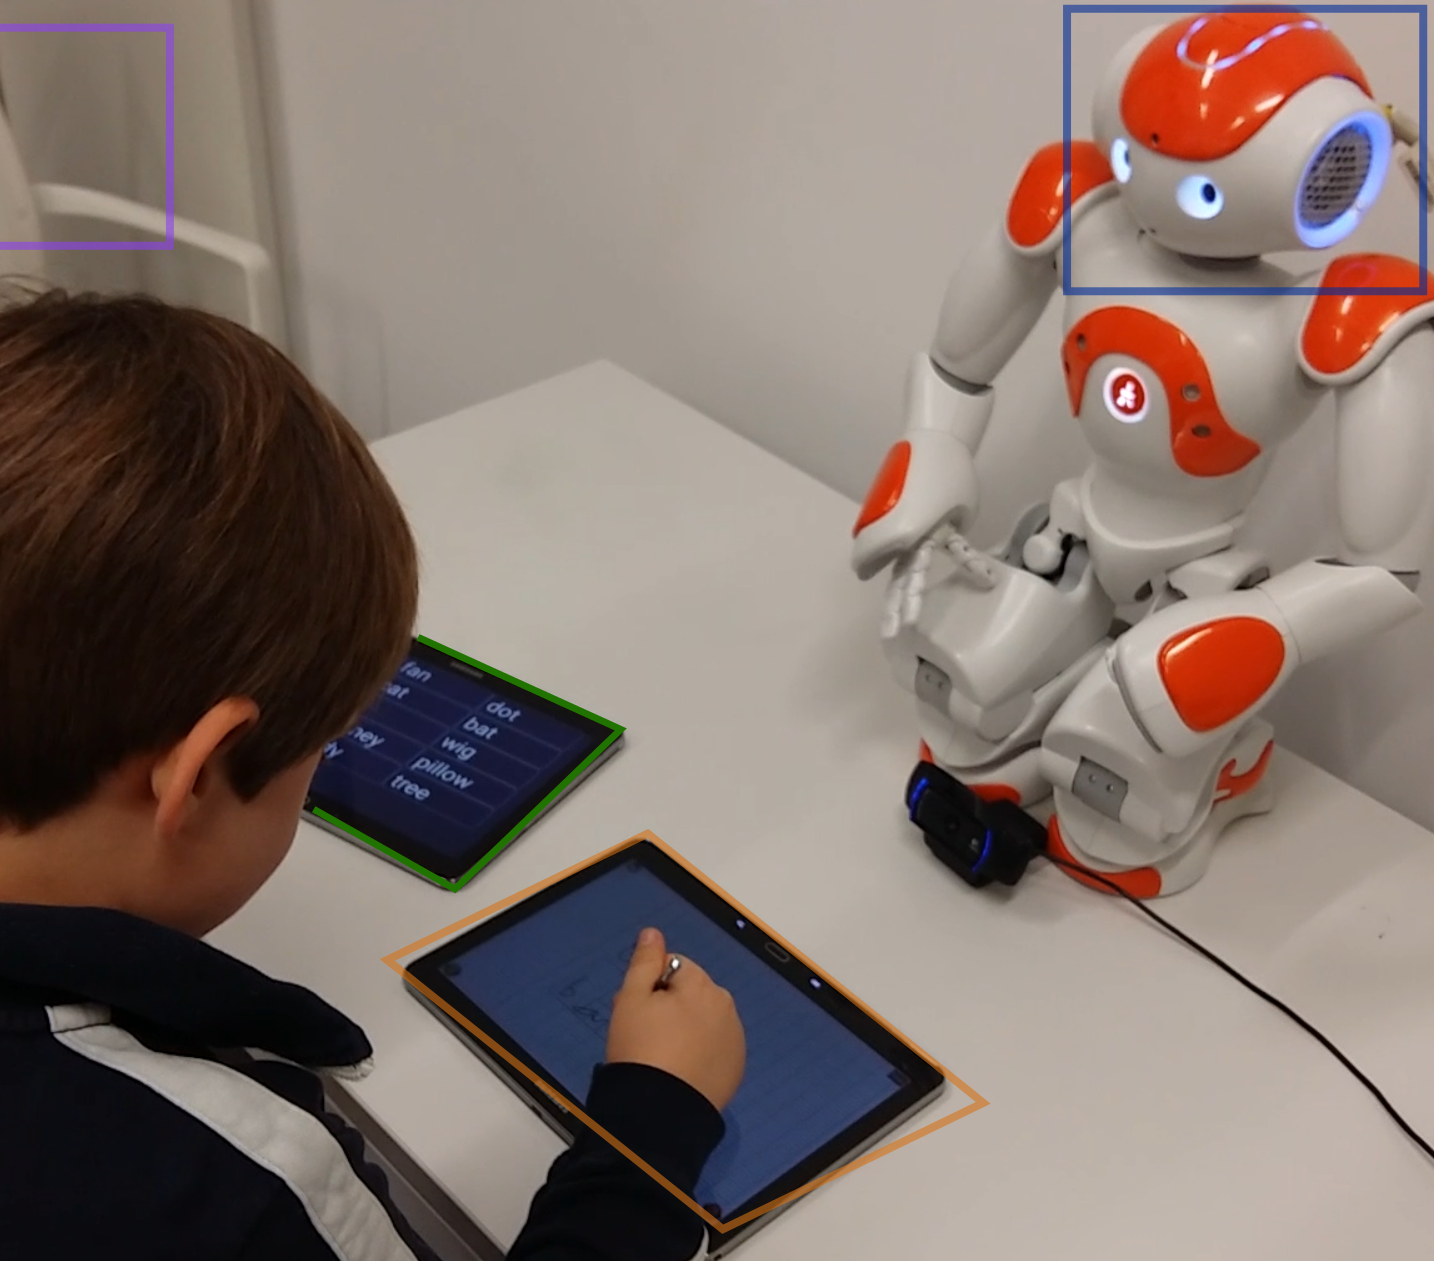
\includegraphics[width=0.7\linewidth]{./figures/f2f_photot.png}
  \caption{Face to face spatial formation}
  \label{fig:sub1}
\end{subfigure}%
\begin{subfigure}{0.5\textwidth}
  \centering
  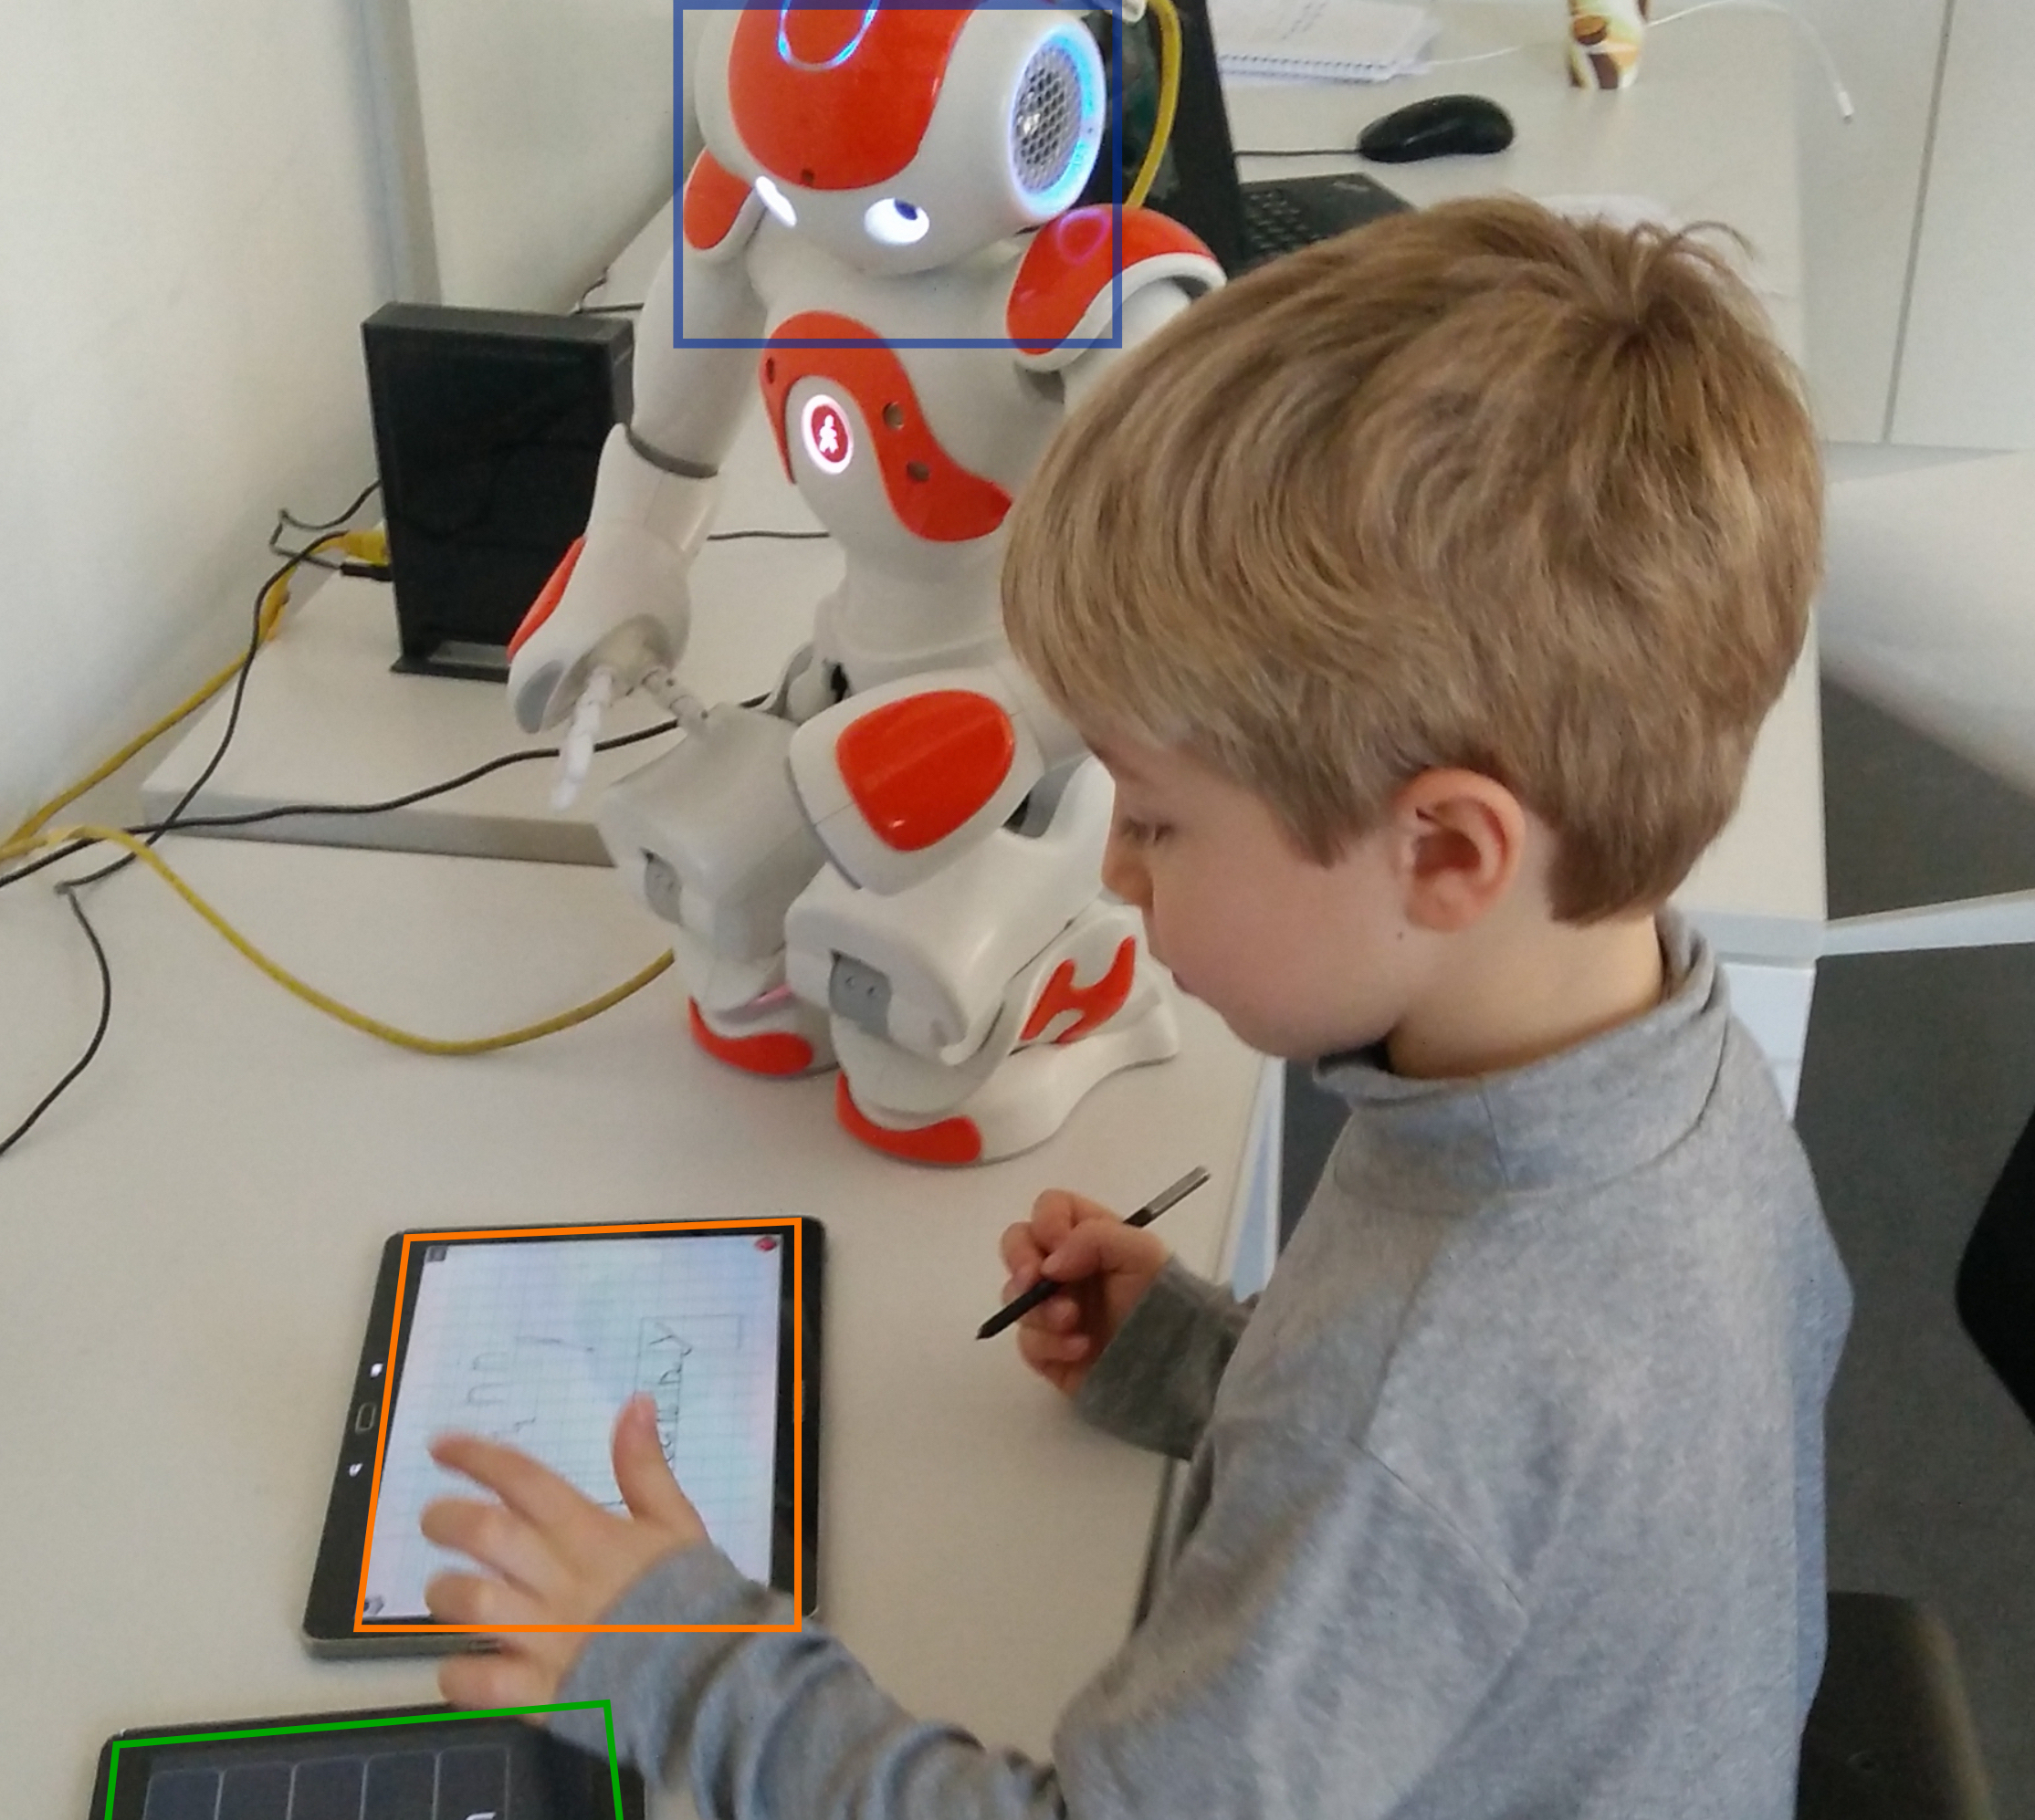
\includegraphics[width=0.7\linewidth]{./figures/s2s_photo2t.jpg}
  \caption{Side by Side spatial formation}
  \label{fig:sub2}
\end{subfigure}
 \caption{Experimental set-ups showing the \emph{with-me-ness} targets in the rectangles: orange - the writing tablet,  blue - the robot's head, green - the tablet used to select a word to teach to the robot}
\label{fig:test}
\end{figure*}

Apart from this change in the spatial setting, the interaction was kept the same. 
The children were told they had to teach the robot how to write some words. 
We briefly presented the two tablet interfaces and the interaction started.
Any word from a list displayed on the selection tablet could be picked by the child.
As the robot would start to write this word. It was set to be a very bad writer at the beginning of the first session for each child.
The child could then give a feedback to the robot by pressing thumbs up or a thumbs down buttons how many times they wanted.
The child would then use a pen and demonstrate how to write the word and the robot would then rewrite the word using the demonstration of the child.
The generated writing of the robot was computed to be halfway from its previous writing state and the new demonstration provided by the child.

Several hypotheses were made concerning the influence of the spatial arrangement on the interaction.
We expected that the gaze behavior of the child would vary according to the spatial configuration.
More gazing at the robot's head would be expected in the face-to-face condition.
Our research question was to measure the degree to which this also influenced the way children behaved as a teacher (were they more or less severe with the robot facing them).
As children give a feedback to the robot for each demonstration, we intend to measure if there is any difference between vis-a-vis and side-by-side regarding this feedback (does the side-by-side condition trigger more positive feedback? or more appropriate feedback?).
%Because of this influence of facing the robot and being able to see its head, we also believed that the robot would be perceived as more competent in the face to face condition and hence collect more positive feedback from the child.
%Indeed some previous studies have shown that social appearance \cite{goetz2003matching} has an influence on the perceived competences.

The degree of  engagement of the child in the task can also be influenced by the arrangement.
For that particular aspect, we will measure the number of repetitions of each word, as well as the with-me-ness, which is discussed in the following section.
Since children were quite young, we choose to not use any self-reported measures or questionnaires.


\subsection{With-me-ness}
The with-me-ness introduced in HRI by \cite{lemaignan2016realtime}, helps to set specific targets during each state of the interaction and to determine whether the user is looking at one of these attentional targets or not.
The algorithm is based on the \textit{d-lib library} that helps to estimate the head pose of the user using a video from a webcam device for instance.
From this head pose, the visual focus of attention (VFoA) is computed.
The inclusion of the targets in the VFoA allows then to compute the \emph{with-me-ness}.
In a simple way, the \emph{with-me-ness} value will increase if the child looks at the specific set of targets, or else it decreases.
This measure allows us to see if the child is engaged in the interaction and is looking at the tablet or the robot's head when he/she is expected to (according to the task).
Indeed, in our learning by teaching activity, the robot has also a hidden pedagogical role. It's progress aim actually to make the child practice and think about his/her own way of writing. 
In that sense, we can set attentional targets as proposed by \cite{sharma2014me} when the \emph{with-me-ness} was first introduced to measure learner's attention to teachers in MOOC videos.

This measure is actually very close to the notion of synchrony already studied in HRI \cite{delaherche2012interpersonal}, where bounding between individuals is reflected by their ability to synchronize in the task (look at the same time at the same targets).

For this experiment, the targets were: "the observer"(a teacher or a teacher assistant),"the experimenter",  "the selection tablet"(the tablet used to pick a word) and the "tablet".
The with-me-ness is initially set to 0.5 and takes values from 0 to 1.
According to the state in which the activity is, (robot is writing, child is writing,\dots) the with-me-ness will be increased if the child looks at a target that is in the set of task-related targets (expected within this particular state of the activity).
We record these targets and the with-me-ness at a frequency of about $1Hz$.
The evolution of the withmeness is computationally attenuated in order to remove noisy data (by using the weighted cumulative of the withmeness value).


The targets were defined according to their spatial relation with the camera used (placed on the table at the robot's feet).
The position of the targets was changed according to the F-formation condition, but the camera stayed at the same position
Figure \ref{fig:test} shows these targets for the two conditions.

\vspace{-0.1cm}
\subsection{Reward Mechanism}
\vspace{-0.2cm}
\label{ss:feedback}
The tablet interface on which the child and the robot practice their handwriting shows two buttons that allow the child to give a positive (green thumb-up) or negative (red thumb-down) feedback to the robot's handwriting.
After every trial of the robot, the child could click on these feedback buttons as much as he/she wants.
We monitored each of these clicks.

These clicks aimed to assess the child's perception of the robot's progress.
When converging to a better writing we expect the child to give better feedback.
However, these buttons could also be used by the child as an encouragement method and children could give a positive feedback even though the robot didn't make progress.

\subsection{Performances}
As the child was managing which word the robot would learn, he/she could also provide as many demonstrations as he/she wanted.
The child was also free to change the word when satisfied with the robot's performance.

\subsubsection{Response Time and Writing Time}
We recorded the time spent on the writing and the response time for each word demonstrated by the children.
We also monitored the number of demonstrations provided by the child for each word.
These measure were cues to how dedicated the child was in the task 

\subsubsection{Writing Score for the Robot}
%Regularity of writing in time
Since the learning algorithm took as input the child's demonstration, if the child provided repeatedly the exact same demonstration, then the robot would converge faster to his/her handwriting.
This score is hence a hint on children's regularity, with the underlying assumption that the regularity in handwriting is a sign of legibility.
%Since children are teaching the robot, they may judge the robot's handwriting according to their provided demonstration, and compare simply their demonstration with the robot's.

At each demonstration of the robot, we were calculating a \emph{writing score}. 
Each demonstration was encoded as a list of seventy 2D points.
This \emph{writing score} is the euclidian distance between the demonstrated letter by the child and the generated letter by the robot.

We also computed the evolution of this score at each demonstration.
We represented the evolution of the robot's handwriting with different states:
'S=': the first trial of this word by the robot, 'S-': the score is decreasing and 'S+' the score is increasing. 
If the child was changing a lot his/her way of writing between consecutives demonstration, the score would then decreasee.
In the contrary, the regularity of the demonstration would make the score increase rapidly.


\section{RESULTS}
%The effect of IV on DV was statistically significant ($F_{a,b}= C, p<d*$). 
%The effect of IV on DV was not statistically significant ($F_{a,b}= C, ns$). 
%In this section, we present results from this study on 12 children that interacted with the robot twice in the two conditions (side-by-side and face-to-face).
%We studied the impact on the F-formation on the reward given with the buttons, the performance and the with-me-ness.

\subsection{Reward Mechanism}
\vspace{-0.2cm}
Children gave feedback with an average of 3 feedbacks per demonstration (i.e. per interaction loop).
We summed the feedbacks for each demo with positive feedback counted as $+1$ and negative as $-1$.
Figure \ref{fig:uf_nb} shows the average evolution along the demonstrations of the sum of feedbacks given for all children and for both spatial condition.
We noticed that the feedback is first negative and grows towards a positive feedback after each demonstration.
In average for all the children, the sum of feedbacks stayed negative until the 5th demonstration.
Children well understood that they were teaching the robot and often gave bad scores for the first untrained trial of the robot.
Children usually gave a positive feedback just before changing the word taught to the robot.

\begin{figure}
	\centering
	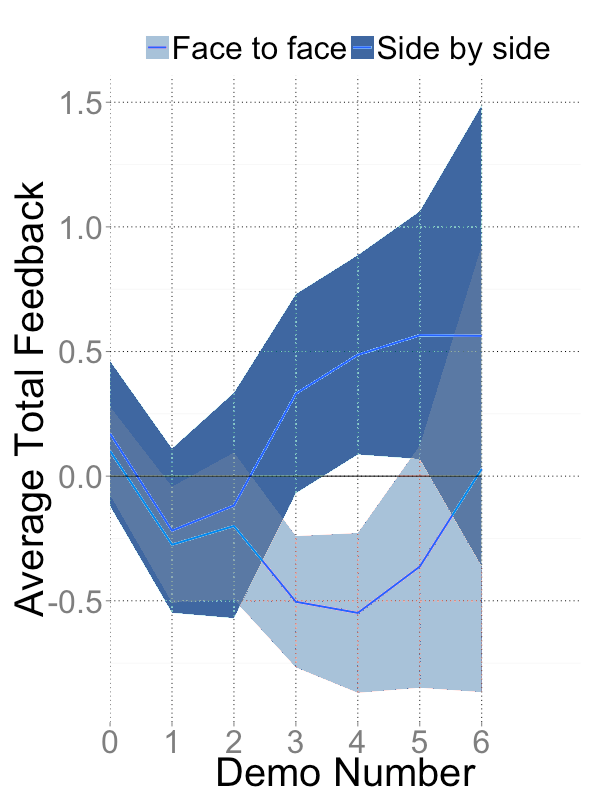
\includegraphics[width=0.75\linewidth]{figures/plots/evoldemocondbis}
	\caption{Evolution of Feedback along the demonstration index(Mean: line , Confidence Interval 0.95: filled area)}
	\label{fig:uf_nb}
\end{figure}
Even though the average feedback was increasing along with the number of demonstration for both condition, they don't seems to increase the same way(see Figure\ref{fig:uf_nb})
The effect of the F-Formation on the feedback from the child was statistically significant (Anova Repeated measures within subjects: $F_{1,272}= 4.396, p<0.05$). As, illustrated on Figure \ref{fig:userfeedback_fformation_se}, the average feedback per demonstration was greater($M=0.03, SD=1, N=147$) for the side-by-side condition compare to the face-to-face condition ($M=-0.23, SD=0.98, N=138$).
 \begin{figure}
 	\centering
 	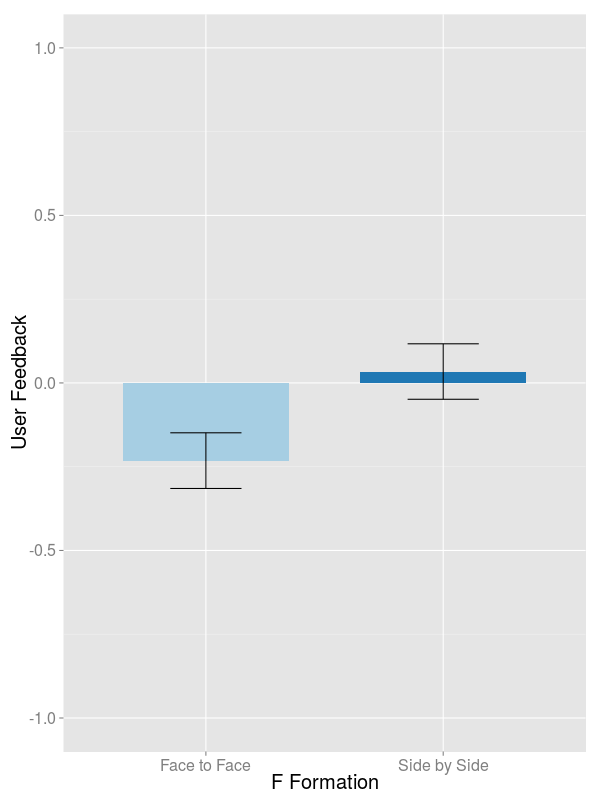
\includegraphics[width=0.58\linewidth]{figures/plots/userfeedback_fformation_se}
 	\caption{Feedback Sum According to the F-Formation (Means and Confidence Intervals)}
 	\label{fig:userfeedback_fformation_se}
 \end{figure}

Children kept giving feedback along the interaction and no drop in the number of feedbacks was observed during the experiment.
They took their duty to teach the robot seriously in that way.

We also observe an order effect showing that children tended to give higher feedback in the second session compare to the first one.
%todo see if adding test
This can simply be explained by the fact that the robot's learning state was progressive between the two session. 
The robot didn't start to learn from scratch in the second session but had already some knowledge from the first session with this same child. 





\subsection{With-me-ness}
\vspace{-0.2cm}
Children understood the dynamics of the interaction, as in general the with-me-ness stayed above 0.5 throughout the interaction (started et 0.5 but always finished above).
\begin{figure}	
\centering
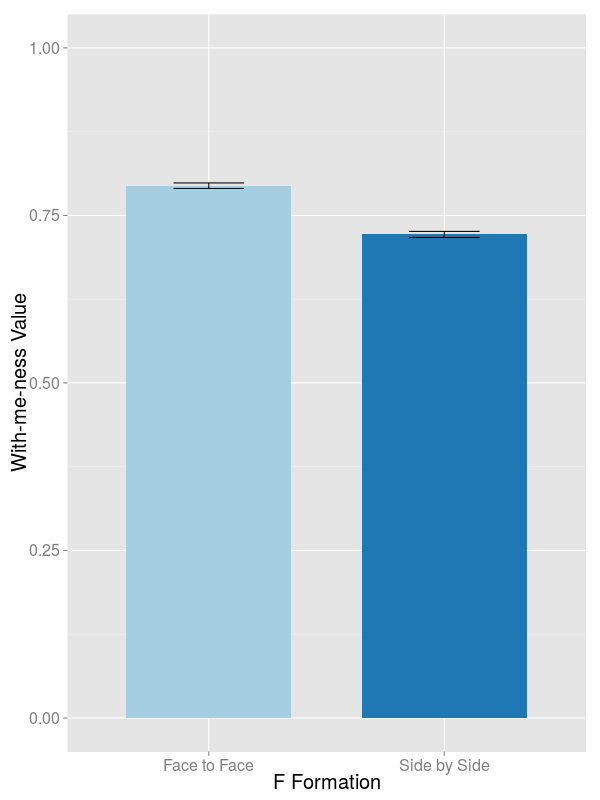
\includegraphics[width=0.6\linewidth]{figures/plots/withmeness_fformation_ci}
\caption{With-me-ness According to the F-Formation (Means and Confidence Intervals)}
\label{fig:withmeness_fformation_ci}

\end{figure}
 The effect of the F-Formation on the with-me-ness of the child was statistically significant (Anova Repeated measures within subjects: $F_{1,15983}= 293.2, p<0.001$). The with-me-ness was greater($M=0.79, SD=0.18, N=7722$) for the face-to-face condition compare to the side-by-side condition ($M=-0.72, SD=0.21, N=8267$) (see Figure \ref{fig:withmeness_fformation_ci}).
 This result was expected, as the robot was facing the robot, its face was more visible for the child.


Again, we observed an order effect with the withmeness increasing between the two sessions. 
As children were more confordable with the system, it is logic that they started to learn the dynamics of the interaction knowing when to look at the selection tablet, the writing tablet and the robot. 
%todo add stats
%	session	N	new_w	sd	se	ci
%	1	1	8886	0.7248584	0.2175269	0.002307596	0.004523421
%	2	2	7103	0.7965673	0.1691839	0.002007419	0.003935140
%Error: Within
%Df Sum Sq Mean Sq F value Pr(>F)    
%session       1   12.8  12.797   339.8 <2e-16 ***
%Residuals 15985  602.0   0.038        

\subsection{Performances}
%\begin{figure}
%\centering
%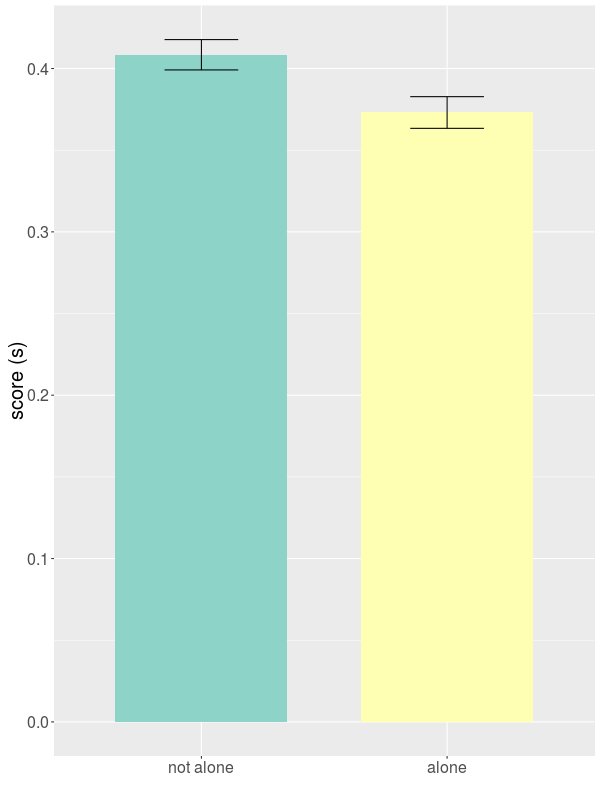
\includegraphics[width=0.4\linewidth]{figures/plots/score_alone_se}
%\caption{Learning speed According to group or alone modality}
%\label{fig:score_alone_ci}
%\end{figure}
\subsubsection{Response Time and Writing Time}
Figure \ref{fig:times} shows on the left the average number of demonstration for each word taught to the robot for the two spatial arrangement conditions. 
There was no significant difference between the conditions even-though the average number of demonstration given by the child in the side-by-side condition seems higher than the face-to-face.

The center graph of Figure \ref{fig:times} shows the average response time for the demonstration provided by the children for the two spatial arrangement conditions.
The response time is the delay between the time when the robot finishes to write and the time when the child touches the tablet.
There was no significant difference between the conditions.
% ($F(1,11)=0, p=0.986$).
 
The writing time (right graph on Figure \ref{fig:times}) corresponds to the delay between the time when the robot finishes its trial and the time the child finishes its new demonstration or changes word. This time also include the moment in which the child can give a feedback via the buttons.
No significant difference in the writing time was found.
%($F(1,11)=1.507, p=0.24$). 

\begin{figure*}[ht]
	\centering
	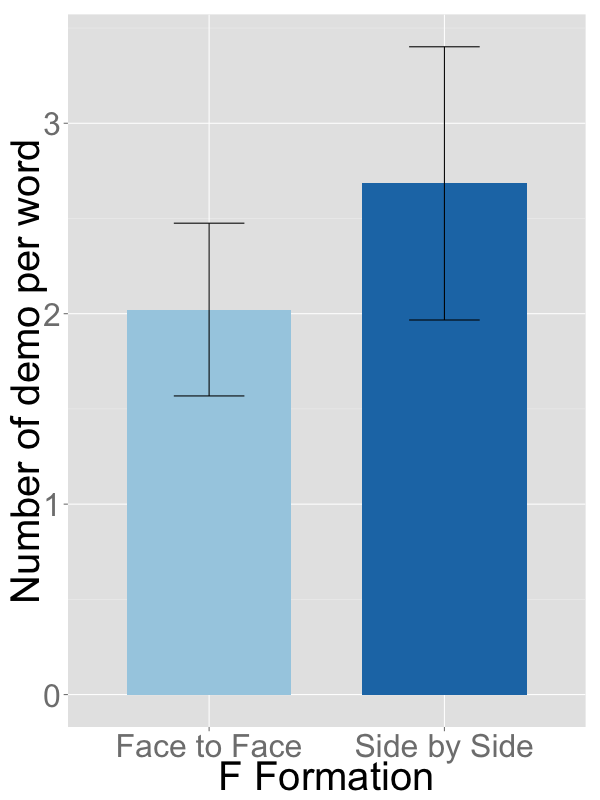
\includegraphics[width=0.25\linewidth]{figures/plots/repetition_fformation_ci}
	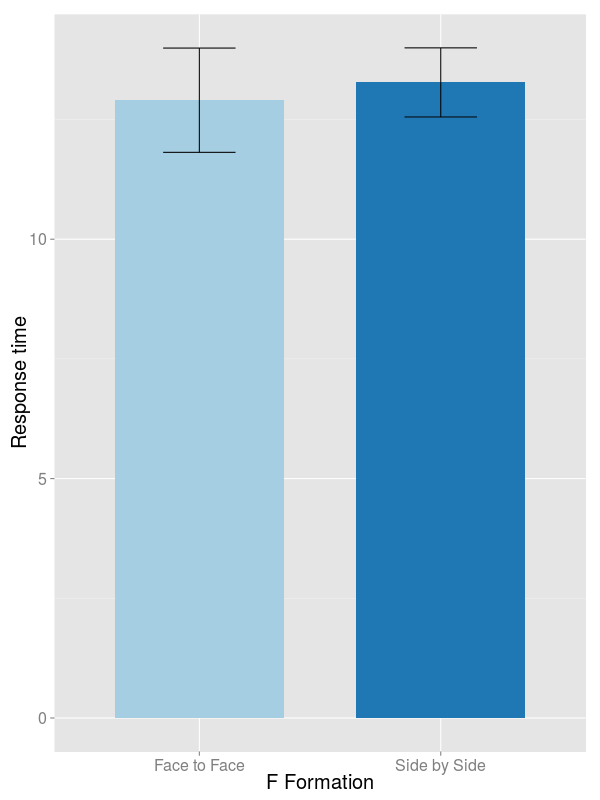
\includegraphics[width=0.25\linewidth]{figures/plots/responseTime_fformation_ci}
	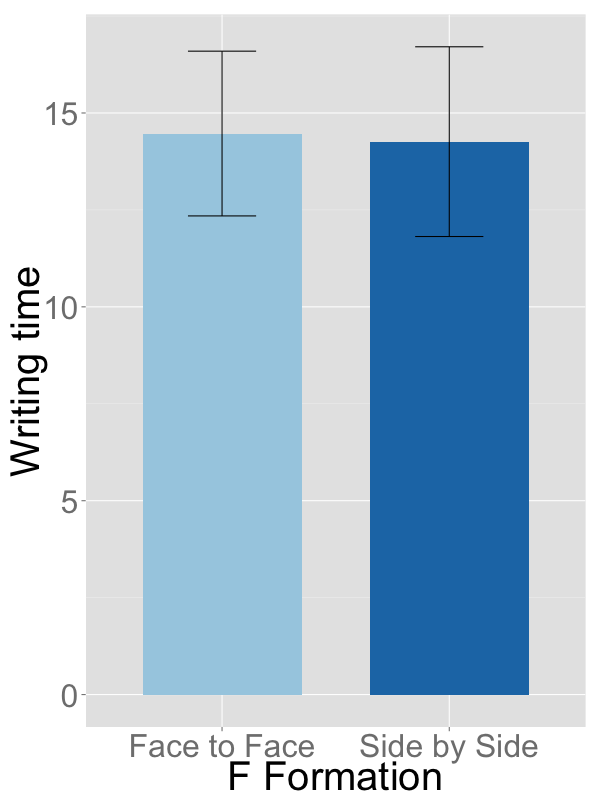
\includegraphics[width=0.25\linewidth]{figures/plots/writingTime_fformation_ci2}
	\caption{Number of demonstration per word (left), response time (center), writing time (right) - (Means and Confidence Intervals)}
	\label{fig:times}
	\end{figure*}

These results show that children when not spending more time per word in one condition of the other. 
The spatial condition didn't influence the involvement of the child in the task. 
% The effect of the group variable on the score of the child was statistically significant ( $F_{1,279}= 6.928, p<0.01$). The score was greater($M=0.41, SD=0.11, N=141$) in  the alone condition compare to the group condition ($M= 0.37, SD=0.11, N=140$).
%These results confirm the fact that the robot is better suited here for individual interaction. 
\subsubsection{Writing Score for the Robot}
There was no significant difference of writing score in the F-formation condition tested (side-by-side:$M=0.80, SD=0.08, N=135$, face-to-face: $M=0.79, SD=0.08, N=191$, Anova Repeated measures within subjects:$p>0.1$).
This result means that the children were teaching as well in the face-to-face condition as in the side-by-side condition.
However, results showed significant differences in terms of feedback given to the robot regarding the score of the robot.

We analyzed the probabilities of succeeding events considering feedback events and score evolution events.

Table~\ref{proba} shows the probabilities of transition from after the score increases and after the score decreases.
We notice that in general the positive feedback probabilities are higher for the side-by-side condition in comparison to the face-to-face. 
On the contrary, the probability of having a negative feedback after is higher in the face-to-face condition.
We can also notice that when the score decreases, the probability of having a positive feedback is almost twice higher in the side-by-side condition (total number of events $= $).


\begin{table}[ht!]
\centering
\caption{\small Probability of feedback given the score per word in  the two conditions : face-to-face / \emph{side-by-side}}
\label{proba}
\begin{tabular}{l|p{1.3cm}|p{1.3cm}|p{1.2cm}}
\toprule
\backslashbox{Score Event}{Feedback} & Positive  & Negative & None \\
\midrule
Score Increases & 	0.37 / \emph{0.44}	& 0.39 / \emph{0.27} & 0.24 / \emph{0.29} \\
Score Decreases &	0.28 / \emph{0.47}	& 0.36 / \emph{0.20} & 0.36 / \emph{0.33} \\
\bottomrule
\end{tabular}
\end{table}

\begin{figure*}
	\centering
	\begin{subfigure}{0.5\textwidth}
		\centering
		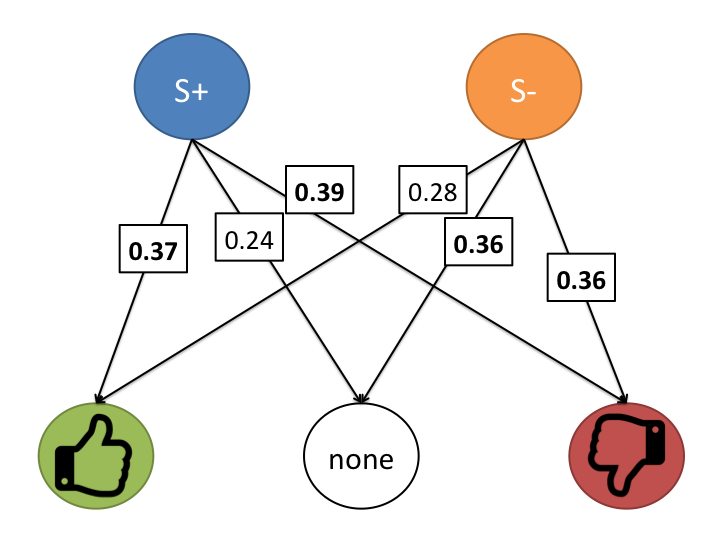
\includegraphics[width=0.8\linewidth]{./figures/states/states_f2f}
		\caption{Face to face spatial formation}
		\label{fig:f2fstate}
	\end{subfigure}%
	\begin{subfigure}{0.5\textwidth}
		\centering
		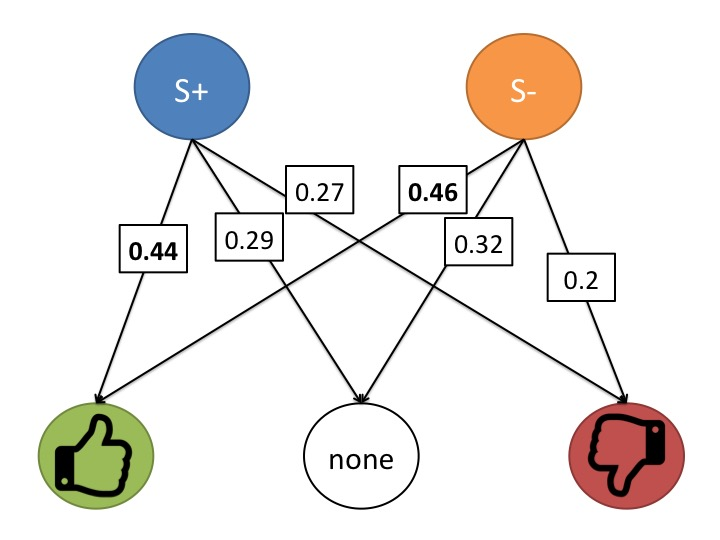
\includegraphics[width=0.8\linewidth]{./figures/states/statess_sbs}
		\caption{Side by Side spatial formation}
		\label{fig:sbsstate}
	\end{subfigure}
	\caption{Transitions states from score evolutions ($S+$ : score increasing compared to previous score, $S-$: score decreasing compare to the previous) to children's feedback (thumb up: positive feedback, thumb down : negative feedback, and no feedback given)}
	\label{fig:state}
\end{figure*}

All the transitions between the scores and the feedback buttons are illustrated on Figure \ref{fig:state}.
Children were displaying a more positive attitude towards the robot when placed in side-by-side position even when the robot was not improving.
This positive attitude was showed by rewarding more improvements of the robot and also penalizing less the retrogression of the robot's writing.
Children even rewarded retrogression more often in the side-by-side condition.
The reward given by children showed to be not often appropriate. 
For instance in the face-to-face condition, score increasing got more than a third of the time given a negative feedback.
These differences in the transition matrix were not significant (Pearson's Chi-squared test, $X-squared = 30, df = 25, p-value = 0.2243$) and a study with a larger number of participants might have given more precise results.



\section{DISCUSSIONS AND CONCLUSIONS}
\vspace{-0.1cm}
In this paper we presented a study that aimed to elicit the effect of spatial arrangement on a learning task between a robot and a child.
Spatial configuration has never to our knowledge been studied in terms of effect on the task but usually in the context of the social interaction.
In this experiment, we showed that this spatial arrangement could also have an influence in the task and on how the child was behaving as a teacher.
Our results showed that even if the robot's learning didn't vary between the side-by-side and the face-to-face condition, the feedback from the child was varying.
This suggests that the relationship between the child and the robot was different between the conditions.
These results are in line with the literature in spatial arrangement and non-verbal social cues.

While running the experiments, we noticed that the children were expecting the robot to react to the feedback, and the robot was moving only when writing. 
We are working on different form of reactions for future experiments to allow the robot to react according to the feedback from the child and also in perspective with the fairness of the feedback regarding the score of the robot.
For instance, if the child gives a positive feedback when the robot is actually improving, the robot should display a positive emotion.
If it is given a positive feedback but does not actually make any progress, it might express doubt to force the child to be more exigent. 


Even if our results showed that the side-by-side elicited more positive feedback from the children, statistical significance was not reached, and if the robot would display some emotional reaction during the interaction, the same effect might not be observed. 
We plan to enhance the interaction with some behavioral reaction and to research the effect of such reactions on the child's perception of the robot's progresses. 
Long term studies might also bring more insights to theses results in order to see if the effect of the spatial arrangement sustain over time.

To conclude, we believe that spatial arrangement can be used as a non-verbal cue of communication to contextualize the interaction (as cooperative or competitive for instance).
%discuss results regarding the literature, same ? different arguments for/against initial premise, limitations, etc.





%\addtolength{\textheight}{-12cm}   % This command serves to balance the column lengths
                                  % on the last page of the document manually. It shortens
                                  % the textheight of the last page by a suitable amount.
                                  % This command does not take effect until the next page
                                  % so it should come on the page before the last. Make
                                  % sure that you do not shorten the textheight too much.

%%%%%%%%%%%%%%%%%%%%%%%%%%%%%%%%%%%%%%%%%%%%%%%%%%%%%%%%%%%%%%%%%%%%%%%%%%%%%%%%



%%%%%%%%%%%%%%%%%%%%%%%%%%%%%%%%%%%%%%%%%%%%%%%%%%%%%%%%%%%%%%%%%%%%%%%%%%%%%%%%



%%%%%%%%%%%%%%%%%%%%%%%%%%%%%%%%%%%%%%%%%%%%%%%%%%%%%%%%%%%%%%%%%%%%%%%%%%%%%%%%
\vspace{-0.1cm}
\section*{ACKNOWLEDGMENT}
\vspace{-0.2cm}
\small
This research was partially supported by the Funda\c{c}\~{a}o para a Ci\^{e}ncia
e a Tecnologia (FCT) with reference UID/CEC/ 50021/2013, and by the Swiss
National Science Foundation through the National Centre of Competence in
Research Robotics.



%%%%%%%%%%%%%%%%%%%%%%%%%%%%%%%%%%%%%%%%%%%%%%%%%%%%%%%%%%%%%%%%%%%%%%%%%%%%%%%%



\small
\bibliographystyle{abbrv}
\bibliography{fformation_cowriter}


\end{document}
